\chapter{Trabajos relacionados}


\section{Consideraciones iniciales}
Reconocer el movimiento humano sin etiquetas es un problema difícil de visión por computadora que ha sido el foco de una gran cantidad de investigación. Muchos enfoques diferentes en este campo abarcan un amplio espectro de técnicas, desde el seguimiento del cuerpo completo en 3D con múltiples cámaras hasta modelos de inferencia bayesiana. Los métodos también varían mucho en los requisitos computacionales, de modo que una solución que es más precisa puede ser prácticamente inutilizable para aplicaciones en tiempo real o para un motor de búsqueda que se utilizará en un sistema CBVR.

\section{Descripcion de los trabajos}

\subsection{Trayectorias spatio-temporal}
En esta sección definimos el template spacio-temporal que utilizaremos el cual es llamada MVFI(Motion vector Flow Instance) 
\subsubsection{Template spatio-temporal  MVFI}
se describe el template spatio-temporal MVFI, que codifica el campo de velocidad de diferentes movimientos humanos. Estas plantillas, correspondientes a cada trama de imagen, se construye trazando el campo de flujo óptico, f, del movimiento de primer plano sobre una rejilla uniformemente espaciada, dada por $x_n$, $y_m$. En cada punto de cuadrícula $x_i$; $y_j$, se codifican la magnitud y la dirección del vector de flujo óptico $v_{ij}$. La dirección por un cuadro delimitador, mientras que la magnitud por el color del píxel (figura \ref{fig:2}). \\
Para un vídeo de entrada que consta de tramas $N_f$, este procedimiento producirá una secuencia de vídeo correspondiente de frames de plantilla que teniendo $N_{f-1}$ (figura \ref{fig:2}) ilustra estos conceptos y muestra el esquema de codificación MVFI para el flujo óptico denso de una secuencia de vídeo.
 
 
(figura \ref{fig:2})muestra la idea básica de cómo se construye el MVFI con un video de boxeo. Para la ejemplificación, los vectores ópticos de flujo correspondientes se superponen sobre en un frame en particular en la secuencia de vídeo. Una explicación más detallada del algoritmo de formación de template es la siguiente: una lista de almacenamiento vacía \textit{l}, utilizada como contenedor temporal para manipular vectores \textbf{f} en el instante \textit{t}. Para cada punto de la grid de flujo óptico $x_i$, $y_j$, la información sobre el vector se utiliza para formar los boxes que se insertan en la lista \textit{l}. A continuación, esta lista \textit{l} se clasifica por tamaño de los box, para que los box más grandes esten en la parte superior. Para construir las plantillas de imagen finales en cada momento, \textbf{t}, loz boxez se separan de la lista ordenada \textit{l} y son dibujados dentro de un frame de imagen vacía. De esta forma, la plantilla acentúa los componentes de velocidad más grandes colocando estos vectores en la parte superior, los cuales serán visibles en la plantilla secuencia. Este mismo procedimiento se repite para todos los cuadros de imagen subsiguientes en la toma de video.
 
 
\begin{figure}
\label{fig:2}
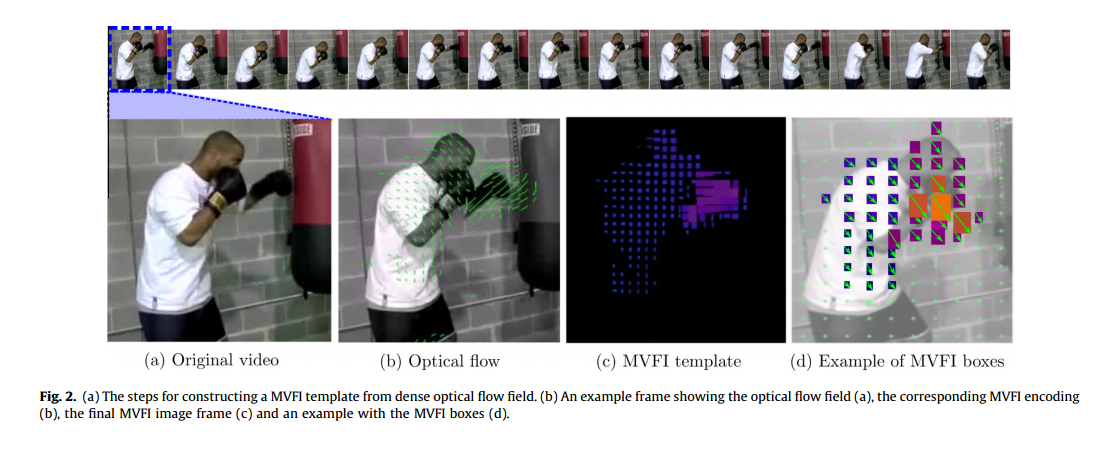
\includegraphics[width=1.0\linewidth]{Kap2/img/Selection_021.png}
\caption{cambiar}
\end{figure}

%\section{Comparación de los trabajos}

%\section{Consideraciones finales}

 

 


